\documentclass[11pt,a4paper]{report}
\usepackage[textwidth=37em,vmargin=30mm]{geometry}
\usepackage{calc,xunicode,amsmath,amssymb,paralist,enumitem,tabu,booktabs,datetime2,xeCJK,xeCJKfntef,listings}
\usepackage{tocloft,fancyhdr,tcolorbox,xcolor,graphicx,eso-pic,xltxtra,xelatexemoji}

\newcommand{\envyear}[0]{2025}
\newcommand{\envdatestr}[0]{2025-01-07}
\newcommand{\envfinaldir}[0]{webdb/2025/20250107/final}

\usepackage[hidelinks]{hyperref}
\hypersetup{
    colorlinks=false,
    pdfpagemode=FullScreen,
    pdftitle={Web Digest - \envdatestr}
}

\setlength{\cftbeforechapskip}{10pt}
\renewcommand{\cftchapfont}{\rmfamily\bfseries\large\raggedright}
\setlength{\cftbeforesecskip}{2pt}
\renewcommand{\cftsecfont}{\sffamily\small\raggedright}

\setdefaultleftmargin{2em}{2em}{1em}{1em}{1em}{1em}

\usepackage{xeCJK,xeCJKfntef}
\xeCJKsetup{PunctStyle=plain,RubberPunctSkip=false,CJKglue=\strut\hskip 0pt plus 0.1em minus 0.05em,CJKecglue=\strut\hskip 0.22em plus 0.2em}
\XeTeXlinebreaklocale "zh"
\XeTeXlinebreakskip = 0pt


\setmainfont{Brygada 1918}
\setromanfont{Brygada 1918}
\setsansfont{IBM Plex Sans}
\setmonofont{JetBrains Mono NL}
\setCJKmainfont{Noto Serif CJK SC}
\setCJKromanfont{Noto Serif CJK SC}
\setCJKsansfont{Noto Sans CJK SC}
\setCJKmonofont{Noto Sans CJK SC}

\setlength{\parindent}{0pt}
\setlength{\parskip}{8pt}
\linespread{1.15}

\lstset{
	basicstyle=\ttfamily\footnotesize,
	numbersep=5pt,
	backgroundcolor=\color{black!5},
	showspaces=false,
	showstringspaces=false,
	showtabs=false,
	tabsize=2,
	captionpos=b,
	breaklines=true,
	breakatwhitespace=true,
	breakautoindent=true,
	linewidth=\textwidth
}






\newcommand{\coverpic}[2]{
    % argv: itemurl, authorname
    Cover photo by #2~~(\href{#1}{#1})
}
\newcommand{\makeheader}[0]{
    \begin{titlepage}
        % \newgeometry{hmargin=15mm,tmargin=21mm,bmargin=12mm}
        \begin{center}
            
            \rmfamily\scshape
            \fontspec{BaskervilleF}
            \fontspec{Old Standard}
            \fontsize{59pt}{70pt}\selectfont
            WEB\hfill DIGEST
            
            \vfill
            % \vskip 30pt
            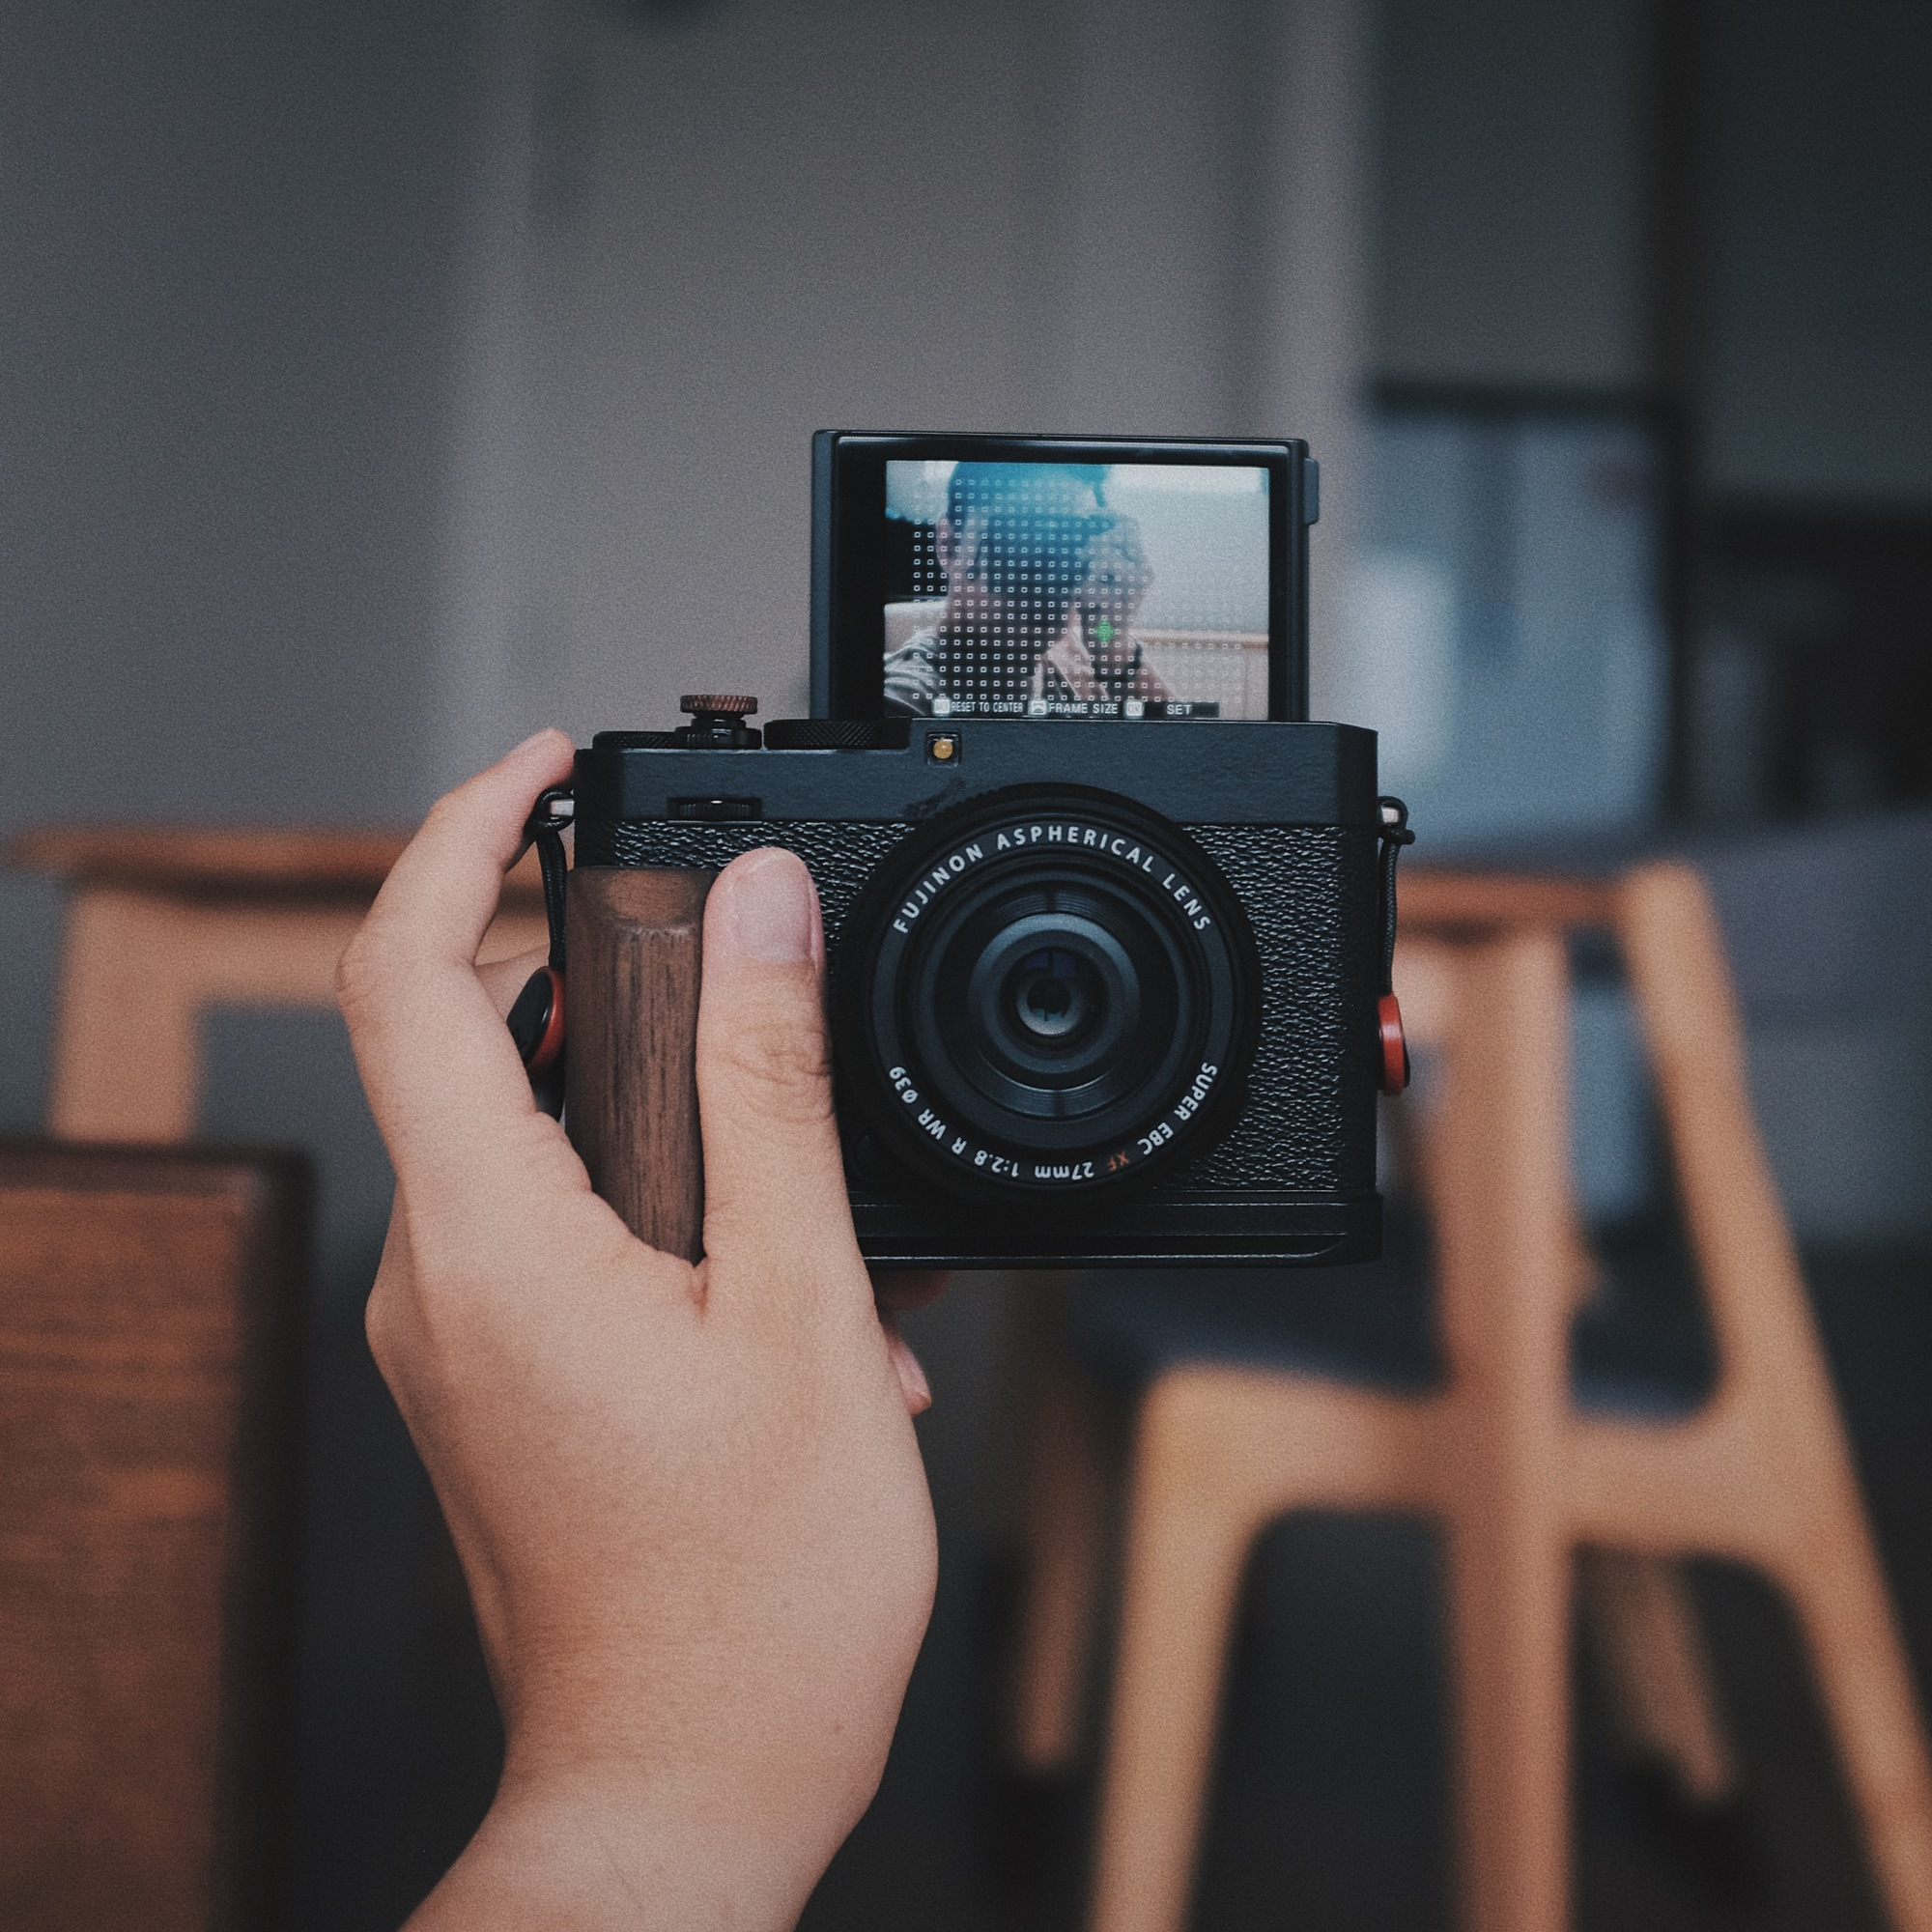
\includegraphics[width=\linewidth]{\envfinaldir/coverpic-prod.jpg}\par
            % \vskip 30pt
            \vfill

            \normalsize\rmfamily\scshape
            \copyright{} The Web Digest Project \hfill\large \envdatestr
        \end{center}
    \end{titlepage}
    % \restoregeometry
}
\newcommand{\simplehref}[1]{%
    \textcolor{blue!80!green}{\href{#1}{#1}}%
}
\renewcommand{\contentsname}{\center\Huge\sffamily\bfseries Contents\par\vskip 20pt}
\newcounter{ipartcounter}
\setcounter{ipartcounter}{0}
\newcommand{\ipart}[1]{
    % \vskip 20pt
    \clearpage
    \stepcounter{ipartcounter}
    \phantomsection
    \addcontentsline{toc}{chapter}{#1}
    % \begin{center}
    %     \Huge
    %     \sffamily\bfseries
    %     #1
    % \end{center}
    % \vskip 20pt plus 7pt
}
\newcounter{ichaptercounter}
\setcounter{ichaptercounter}{0}
\newcommand{\ichapter}[1]{
    % \vskip 20pt
    \clearpage
    \stepcounter{ichaptercounter}
    \phantomsection
    \addcontentsline{toc}{section}{\numberline{\arabic{ichaptercounter}}#1}
    \begin{center}
        \Huge
        \sffamily\bfseries
        #1
    \end{center}
    \vskip 20pt plus 7pt
}
\newcommand{\entrytitlefont}[1]{\subsection*{\raggedright\Large\sffamily\bfseries#1}}
\newcommand{\entryitemGeneric}[2]{
    % argv: title, url
    \parbox{\linewidth}{
        \entrytitlefont{#1}\par\vskip 5pt
        \footnotesize\ttfamily\mdseries
        \simplehref{#2}
    }\vskip 11pt plus 11pt minus 1pt
}
\newcommand{\entryitemGithub}[3]{
    % argv: title, url, desc
    \parbox{\linewidth}{
        \entrytitlefont{#1}\par\vskip 5pt
        \footnotesize\ttfamily\mdseries
        \simplehref{#2}\par\vskip 5pt
        \small\rmfamily\mdseries#3
    }\vskip 11pt plus 11pt minus 1pt
}
\newcommand{\entryitemAp}[3]{
    % argv: title, url, desc
    \parbox{\linewidth}{
        \entrytitlefont{#1}\par\vskip 5pt
        \footnotesize\ttfamily\mdseries
        \simplehref{#2}\par\vskip 5pt
        \small\rmfamily\mdseries#3
    }\vskip 11pt plus 11pt minus 1pt
}
\newcommand{\entryitemHackernews}[3]{
    % argv: title, hnurl, rawurl
    % \parbox{\linewidth}{
    %     \entrytitlefont{#1}\par\vskip 5pt
    %     \footnotesize\ttfamily\mdseries
    %     \simplehref{#3}\par
    %     \textcolor{black!50}{\href{#2}{#2}}
    % }\vskip 11pt plus 11pt minus 1pt
    \begin{minipage}{\linewidth}
            \entrytitlefont{#1}\par\vskip 5pt
            \footnotesize\ttfamily\mdseries
            \simplehref{#3}\par
            \textcolor{black!50}{\href{#2}{#2}}
    \end{minipage}\par\vskip 11pt plus 11pt minus 1pt
}







\begin{document}

\makeheader

\tableofcontents\clearpage




\ipart{Developers}
\ichapter{Hacker News}
\entryitemTwoLinks{Used Meta AI, now Instagram is using my face on ads targeted at me}{https://news.ycombinator.com/item?id=42615538}{https://old.reddit.com/r/ABoringDystopia/comments/1ht7fft/used\_meta\_ai\_to\_edit\_a\_selfie\_now\_instagram\_is/}

\entryitemTwoLinks{An autumn bike adventure down the US portion of the Eastern Divide Trail}{https://news.ycombinator.com/item?id=42613878}{https://www.crazyguyonabike.com/doc/?doc\_id=26078}

\entryitemTwoLinks{C: Simple Defer, Ready to Use}{https://news.ycombinator.com/item?id=42613671}{https://gustedt.wordpress.com/2025/01/06/simple-defer-ready-to-use/}

\entryitemTwoLinks{Software is eating the world, all right (2024)}{https://news.ycombinator.com/item?id=42613550}{https://medium.com/@metapgmr/software-is-eating-the-world-all-right-faedbab6d623}

\entryitemTwoLinks{The Future of Htmx}{https://news.ycombinator.com/item?id=42613221}{https://htmx.org/essays/future/}

\entryitemTwoLinks{All clocks are 30 seconds late}{https://news.ycombinator.com/item?id=42612842}{https://victorpoughon.fr/all-clocks-are-30-seconds-late/}

\entryitemTwoLinks{3blue1brown YouTube Bitcoin video taken down as copyright violation}{https://news.ycombinator.com/item?id=42612494}{https://twitter.com/3blue1brown/status/1876291319955398799}

\entryitemTwoLinks{My little sister's use of ChatGPT for homework is heartbreaking}{https://news.ycombinator.com/item?id=42611844}{https://old.reddit.com/r/ChatGPT/comments/1hun3e4/my\_little\_sisters\_use\_of\_chatgpt\_for\_homework\_is/}

\entryitemTwoLinks{Justin Trudeau promises to resign as PM}{https://news.ycombinator.com/item?id=42611730}{https://www.cbc.ca/news/politics/trudeau-news-conference-1.7423680}

\entryitemTwoLinks{Spline Distance Fields}{https://news.ycombinator.com/item?id=42611540}{https://zone.dog/braindump/spline\_fields/}

\entryitemTwoLinks{Stimulation Clicker}{https://news.ycombinator.com/item?id=42611536}{https://neal.fun/stimulation-clicker/}

\entryitemTwoLinks{Show HN: Mashups – Resurrecting Yahoo Pipes, my side project}{https://news.ycombinator.com/item?id=42609819}{https://www.mashups.io}

\entryitemTwoLinks{Time-Series Anomaly Detection: A Decade Review}{https://news.ycombinator.com/item?id=42609595}{https://arxiv.org/abs/2412.20512}

\entryitemTwoLinks{The evolution of a structural code editor}{https://news.ycombinator.com/item?id=42608923}{https://crowdhailer.me/2025-01-02/the-evolution-of-a-structural-code-editor/}

\entryitemTwoLinks{Lord of the Io\_uring (2020)}{https://news.ycombinator.com/item?id=42608436}{https://unixism.net/loti/index.html}

\entryitemTwoLinks{Uncut Currency}{https://news.ycombinator.com/item?id=42608155}{https://www.usmint.gov/paper-currency/uncut-currency/}

\entryitemTwoLinks{Doom, the Gallery Experience}{https://news.ycombinator.com/item?id=42607794}{https://bobatealee.itch.io/doom-the-gallery-experience}

\entryitemTwoLinks{Hitting OKRs vs. Doing Your Job}{https://news.ycombinator.com/item?id=42607623}{https://jessitron.com/2025/01/05/hitting-okrs-vs-doing-your-job/}

\entryitemTwoLinks{Unemployed office workers are having a harder time finding new jobs}{https://news.ycombinator.com/item?id=42607454}{https://www.wsj.com/economy/jobs/job-search-workers-unemployment-months-5a4cfcee}

\entryitemTwoLinks{Apple squandered the Holy Grail}{https://news.ycombinator.com/item?id=42607151}{https://xeiaso.net/blog/2025/squandered-holy-grail/}\ichapter{Phoronix}
\entryitemGeneric{\hskip 0pt{}AMD Announces Ryzen 9 9950X3D \& Ryzen AI Max, Previews AMD RDNA 4 Graphics}{https://www.phoronix.com/review/amd-ryzen-9950x3d-rdna4-ai-max}

\entryitemGeneric{\hskip 0pt{}DisplayPort 2.1b Arriving This Spring With DP80LL Cables}{https://www.phoronix.com/news/DisplayPort-2.1b-Coming}

\entryitemGeneric{\hskip 0pt{}HDMI 2.2 Announced With 96 Gbps Bandwidth - Still With Restricted Licensing}{https://www.phoronix.com/news/HDMI-2.2-Announced}

\entryitemGeneric{\hskip 0pt{}Qualcomm Bringing Snapdragon X Series To Mini PCs For As Little As ~\$600 USD}{https://www.phoronix.com/news/Qualcomm-Snapdragon-X1-Mini-PCs}

\entryitemGeneric{\hskip 0pt{}Firefox 134 Available With Experimental HTML "autocorrect" Attribute}{https://www.phoronix.com/news/Mozilla-Firefox-134-Available}

\entryitemGeneric{\hskip 0pt{}NVIDIA Working On "-flto-partition=locality" GCC Option To Boost Performance For Some CPU Workloads}{https://www.phoronix.com/news/NVIDIA-GCC-flto-locality}

\entryitemGeneric{\hskip 0pt{}Intel Announces Core Ultra 200H / Core Ultra 200HX Series}{https://www.phoronix.com/news/Intel-Core-Ultra-200H-200HX}

\entryitemGeneric{\hskip 0pt{}Device Mapper Atomic Write Support Patches Posted}{https://www.phoronix.com/news/Device-Mapper-Atomic-Write}

\entryitemGeneric{\hskip 0pt{}Fedora Stakeholders Have Been Debating Whether To Retire GlusterFS}{https://www.phoronix.com/news/Fedora-Maybe-Retire-GlusterFS}


\ipart{Developers~~~~(zh-Hans)}
\ichapter{Solidot}
\entryitemGeneric{\hskip 0pt{}新冠疫情五年之后}{https://www.solidot.org/story?sid=80247}

\entryitemGeneric{\hskip 0pt{}男子被困在在一直绕圈的 Waymo 无人驾驶出租车中}{https://www.solidot.org/story?sid=80246}

\entryitemGeneric{\hskip 0pt{}酒商用无酒精饮料吸引年轻消费者}{https://www.solidot.org/story?sid=80245}

\entryitemGeneric{\hskip 0pt{}雇主以较低的薪酬提供远程办公的灵活性}{https://www.solidot.org/story?sid=80244}

\entryitemGeneric{\hskip 0pt{}FSF 呼吁迁移出 GitHub 以抗议微软 Windows 11 对 TPM2.0 的强制性要求}{https://www.solidot.org/story?sid=80243}

\entryitemGeneric{\hskip 0pt{}微软仍未解决 Windows 11 24H2 与 eSCL 扫描仪的兼容性问题}{https://www.solidot.org/story?sid=80242}

\entryitemGeneric{\hskip 0pt{}网易撤销了对 Linux 和 Mac《漫威争锋》玩家的百年禁令}{https://www.solidot.org/story?sid=80241}

\entryitemGeneric{\hskip 0pt{}闭源浏览器扩展 Pie Adblock 被指抄袭 GPL 授权的 uBlock Origin}{https://www.solidot.org/story?sid=80240}

\entryitemGeneric{\hskip 0pt{}RISC-V 笔记本电脑即将走入生活}{https://www.solidot.org/story?sid=80239}

\entryitemGeneric{\hskip 0pt{}美国卫生局局长呼吁为酒加入致癌警告}{https://www.solidot.org/story?sid=80238}

\entryitemGeneric{\hskip 0pt{}黑客通过钓鱼攻击入侵数十个 Chrome 扩展植入后门}{https://www.solidot.org/story?sid=80237}\ichapter{V2EX}
\entryitemGeneric{\hskip 0pt{}[Telegram] 友友们, telegram 能同时打开多窗口在一个页面上吗?}{https://www.v2ex.com/t/1103051}

\entryitemGeneric{\hskip 0pt{}[问与答] 北京联通有没有老用户可以转的大流量套餐?}{https://www.v2ex.com/t/1103050}

\entryitemGeneric{\hskip 0pt{}[远程工作] [全职远程/卡牌二游] 英国伦敦游戏公司直招 unity 开发工程师}{https://www.v2ex.com/t/1103049}

\entryitemGeneric{\hskip 0pt{}[分享发现] 戴尔发布 2025 新款 UltraSharp 4K 显示器 U2725QE 和 U3225QE}{https://www.v2ex.com/t/1103048}

\entryitemGeneric{\hskip 0pt{}[职场话题] 从面别人,到找不到工作,年底了没脸回家了}{https://www.v2ex.com/t/1103047}

\entryitemGeneric{\hskip 0pt{}[程序员] 正在用 DDD 开发,请问在划分 aggregate 时候,遇到一些多对多的中间表该怎么处理?}{https://www.v2ex.com/t/1103045}

\entryitemGeneric{\hskip 0pt{}[问与答] xdm, emby 削刮没反应怎么办?}{https://www.v2ex.com/t/1103044}

\entryitemGeneric{\hskip 0pt{}[问与答] 关于最近治牙是否合适}{https://www.v2ex.com/t/1103043}

\entryitemGeneric{\hskip 0pt{}[分享创造] 工具分享 | UStars 快捷方便的管理您的 Github Star 项目}{https://www.v2ex.com/t/1103041}

\entryitemGeneric{\hskip 0pt{}[OpenAI] Sam Altman 最新博客(2025.01.05)Reflections}{https://www.v2ex.com/t/1103040}

\entryitemGeneric{\hskip 0pt{}[程序员] 分享一个关于购买的双开微信包有异常风险行为的事情}{https://www.v2ex.com/t/1103038}

\entryitemGeneric{\hskip 0pt{}[随想] 人类的所谓的进步,实际上是退步}{https://www.v2ex.com/t/1103037}

\entryitemGeneric{\hskip 0pt{}[分享创造] 新开发了一个网站,可以用自然语言编辑 Excel,以及生成各种公式}{https://www.v2ex.com/t/1103036}

\entryitemGeneric{\hskip 0pt{}[分享创造] GeneralUpdate 应用程序自动升级跨平台解决方案,支持国产操作系统。}{https://www.v2ex.com/t/1103035}

\entryitemGeneric{\hskip 0pt{}[问与答] 海外回国用腾讯或者阿里云回国是否可行?}{https://www.v2ex.com/t/1103034}

\entryitemGeneric{\hskip 0pt{}[分享发现] CES 2025 即将到来, NVIDIA 和 AMD 也会发布新品,大家有什么购买意愿和想法吗}{https://www.v2ex.com/t/1103033}

\entryitemGeneric{\hskip 0pt{}[VPS] [出] zgo25 刀 9929\&CMIN2, 1h1g20g600g, ip 干净,解锁完美}{https://www.v2ex.com/t/1103032}

\entryitemGeneric{\hskip 0pt{}[Telegram] 发布一个开源项目: Telegram Miniapp Bridge SDK for Unity}{https://www.v2ex.com/t/1103031}

\entryitemGeneric{\hskip 0pt{}[分享创造] Infio-Copilot: 受 Cursor 启发的 Obsidian AI 助手,提供智能自动补全和与选定笔记的交互式聊天}{https://www.v2ex.com/t/1103030}

\entryitemGeneric{\hskip 0pt{}[分享创造] Melody 更新: 支持定时下载歌曲到本地 和 定时备份网易云歌曲到网易云云盘}{https://www.v2ex.com/t/1103029}

\entryitemGeneric{\hskip 0pt{}[程序员] PHP 后端,做独立开发者,怎么弄前端呢?写不了 css,调不了 div 的那种。}{https://www.v2ex.com/t/1103028}

\entryitemGeneric{\hskip 0pt{}[互联网] 哪些手机能无限制安装海外 APP,比如: TG, whatsapp 等}{https://www.v2ex.com/t/1103027}

\entryitemGeneric{\hskip 0pt{}[问与答] alist 对象存储私有域名自签证书一直报错?求解}{https://www.v2ex.com/t/1103026}

\entryitemGeneric{\hskip 0pt{}[宽带症候群] 上海联通千兆宽带阶段性活动}{https://www.v2ex.com/t/1103024}

\entryitemGeneric{\hskip 0pt{}[程序员] 正常求职,什么样的技术水平,才能算得上是资深研发工程师?}{https://www.v2ex.com/t/1103023}

\entryitemGeneric{\hskip 0pt{}[iCloud] iCloud 2T + Apple music 国区拼车}{https://www.v2ex.com/t/1103022}

\entryitemGeneric{\hskip 0pt{}[酷工作] [招聘][远程]英国伦敦公司新开 unity 二次元手游项目}{https://www.v2ex.com/t/1103021}

\entryitemGeneric{\hskip 0pt{}[问与答] ChatGPT 的 Mac 客户端会导致系统卡死}{https://www.v2ex.com/t/1103020}

\entryitemGeneric{\hskip 0pt{}[macOS] Setapp 家庭版 2018 年的老车,组团订阅 2025 年度开始啦}{https://www.v2ex.com/t/1103019}

\entryitemGeneric{\hskip 0pt{}[分享发现] V 友们,有没有便宜的静态住宅 IP 推荐购买网站}{https://www.v2ex.com/t/1103018}

\entryitemGeneric{\hskip 0pt{}[Apple] 初代 iPhone 发布时 499 元,也是一群人喊贵。但现在 499 元只能买到低配版 Pixel 8a。十几年后,会不会 Vision Pro 的 3499 元也成为中低端头显的售价?智能手机和头显一样不是必需品}{https://www.v2ex.com/t/1103016}

\entryitemGeneric{\hskip 0pt{}[全球工单系统] 京东下单时间的 feature}{https://www.v2ex.com/t/1103015}

\entryitemGeneric{\hskip 0pt{}[Android] 三星手机和浏览器字体问题求问}{https://www.v2ex.com/t/1103014}

\entryitemGeneric{\hskip 0pt{}[Steam] 为什么 Steam 客户的聊天无法发图片?}{https://www.v2ex.com/t/1103013}

\entryitemGeneric{\hskip 0pt{}[问与答] 安卓 tv 上有哪些支持播放 smb 上的文件并且比较符合国内交互逻辑的 app?}{https://www.v2ex.com/t/1103012}

\entryitemGeneric{\hskip 0pt{}[问与答] 单 cpu 多核为啥不用并行}{https://www.v2ex.com/t/1103011}

\entryitemGeneric{\hskip 0pt{}[宽带症候群] 发个馒头药}{https://www.v2ex.com/t/1103010}

\entryitemGeneric{\hskip 0pt{}[分享创造] 当了两天的婚恋中介的感受。}{https://www.v2ex.com/t/1103009}

\entryitemGeneric{\hskip 0pt{}[程序员] 如何将一堆 json 文件变成 API 用于接口访问?}{https://www.v2ex.com/t/1103007}

\entryitemGeneric{\hskip 0pt{}[问与答] Jenkins 流程中,构建-部署测试-部署生产,流程时间跨度很长怎么办?}{https://www.v2ex.com/t/1103006}

\entryitemGeneric{\hskip 0pt{}[生活] 为何无故发违停短信?违停短信是摄像头拍到的还是交警操作后发的?}{https://www.v2ex.com/t/1103005}

\entryitemGeneric{\hskip 0pt{}[生活] 看新房子要不要装修的帖子有感}{https://www.v2ex.com/t/1103004}

\entryitemGeneric{\hskip 0pt{}[跑步] 跑步机求推荐}{https://www.v2ex.com/t/1103003}

\entryitemGeneric{\hskip 0pt{}[奇思妙想] 工具网站意见收集箱}{https://www.v2ex.com/t/1103002}

\entryitemGeneric{\hskip 0pt{}[程序员] 现在的 wps 把 Windows 的资源管理器中文件的属性都污染了,怎么办?}{https://www.v2ex.com/t/1103001}

\entryitemGeneric{\hskip 0pt{}[生活] 公司好像集体水逆了}{https://www.v2ex.com/t/1103000}

\entryitemGeneric{\hskip 0pt{}[分享发现] 发现 B 站目前刷到很多白噪音视频,产量稳定,不知道是不是 ai 生成的,有点好奇技术栈}{https://www.v2ex.com/t/1102999}

\entryitemGeneric{\hskip 0pt{}[酷工作] Flashduty 前端实习生(可远程)}{https://www.v2ex.com/t/1102998}

\entryitemGeneric{\hskip 0pt{}[程序员] [教程] 1 分钟微信公众号接入自己的 gpt--官方提供的方案--安全随便造}{https://www.v2ex.com/t/1102997}

\entryitemGeneric{\hskip 0pt{}[分享创造] 分享一款自己写的 Wordpress / Hugo 主题}{https://www.v2ex.com/t/1102996}


\ipart{Generic News}
\ichapter{AP News}
\entryitemWithDescription{\hskip 0pt{}Donald Trump Jr. to visit Greenland as his father muses anew about the US taking control of it}{https://apnews.com/article/7a235a1e756c48ffdb4a3158ced35514}{}

\entryitemWithDescription{\hskip 0pt{}Monkey in a tutu escapes from a home. Missouri sheriff's office says the capture was `bananas'}{https://apnews.com/article/ac4d8d1271755d2f78a6ac64188c1d26}{}

\entryitemWithDescription{\hskip 0pt{}Zendaya sparks engagement speculation at Golden Globes with a sparkling ring}{https://apnews.com/article/6377a46e01e3e24bd1627a130bf3ec73}{}

\entryitemWithDescription{\hskip 0pt{}What to know about the Meta glasses the New Orleans attacker used to scout the French Quarter}{https://apnews.com/article/cf0f94a8ed9e21421735adf0d15d312a}{}

\entryitemWithDescription{\hskip 0pt{}Jaguars fire coach Doug Pederson, keep GM Trent Baalke after `best team assembled' wins just 4 games}{https://apnews.com/article/20f47f397e7885c8dd0fce10ac283076}{}

\entryitemWithDescription{\hskip 0pt{}Inside the Golden Globes: What you didn't see on television}{https://apnews.com/article/6856384ad8702326885542d9585d20c9}{}

\entryitemWithDescription{\hskip 0pt{}Golden Globes Fashion: Ariana Grande eschews Glinda pink for pale yellow (brick road) silk}{https://apnews.com/article/4c71219b0fc6846e944b7a8404b5152a}{}

\entryitemWithDescription{\hskip 0pt{}Lions beat Vikings 31-9, win NFC North and No. 1 seed, dropping division rivals to No. 5}{https://apnews.com/article/d116a1ae8134b4fc3e704894c37b51f7}{}

\entryitemWithDescription{\hskip 0pt{}Lawsuit alleges Skip Bayless harassed Fox Sports hairstylist and offered her \$1.5M for sex}{https://apnews.com/article/5a2a5a8ceb928b8013d46d78287046d4}{}

\entryitemWithDescription{\hskip 0pt{}A soccer-loving nun from Brazil is now the world's oldest living person}{https://apnews.com/article/9428ea98d6d2acb0e234a4390404990b}{}

\entryitemWithDescription{\hskip 0pt{}1 person killed in large avalanche in western Wyoming backcountry}{https://apnews.com/article/cf957d7904dca41184e10289655eb651}{}

\entryitemWithDescription{\hskip 0pt{}A Melania Trump documentary from director Brett Ratner will be released by Amazon}{https://apnews.com/article/fc36fc99e3eff0a18ef8b72335af88f6}{}

\entryitemWithDescription{\hskip 0pt{}Joe Burrow and the Cincinnati Bengals keep their playoff hopes alive by edging the Steelers 19-17}{https://apnews.com/article/e5ae4c470cc87af14c1a377098c72e2b}{}\ichapter{联合早报}
\entryitemWithDescription{沈泽玮:台湾冲突阻遏法案只叫不咬?}{https://www.zaobao.com/news/china/story20240918-4758889}{美国众议院9月9日开启了长达一星期的``中国周'',共通过25项主要涉华法案。(法新社) 美国众议院在当地时间9月9日开启了长达一星期的``中国周'',在美国总统和国会选举举行之前,密集表决数十项与中国有关的法案,共通过25项主要涉华法案……}

\entryitemWithDescription{欧盟电动车关税投票倒计时 中国在分歧中寻支持}{https://www.zaobao.com/news/china/story20240917-4758953}{欧盟27个成员国将于9月25日就是否继续对进口自中国的电动汽车额外征税进行最后表决。图为上海港等待装运出口的电动汽车。(彭博社) 欧盟对中国电动汽车加征关税的投票进入倒计时,正在欧洲访问的中国商务部部长王文涛与欧盟多国政府高层就此进行协商,试图在立场分歧的成员国中争取到更多支持。 受访学者研判,欧盟对中国电动汽车加征关税不可避免,但具体的加税方式和幅度仍有一定弹性,这是王文涛此行与各国谈判的重点……}

\entryitemWithDescription{港府今年将举办逾400项国庆活动}{https://www.zaobao.com/news/china/story20240917-4759341}{再过十多天就是中国国庆75周年,香港天星小轮展示``国庆75周年''\,``三天免费搭小轮''等标语迎国庆。(中新社) 再过十多天就是中国国庆75周年,香港特区政府今年将举办逾400项庆祝活动,希望通过一连串活动庆祝国庆,并且弘扬爱国主义教育及刺激消费。 港府星期二(9月17日)召开记者会,介绍各项庆祝国庆活动和特别优惠,涉及出行及吃喝玩乐等领域……}

\entryitemWithDescription{美空军部长:中国大陆军演精密化 为入侵封锁台湾做准备}{https://www.zaobao.com/news/china/story20240917-4759407}{美国空军部长肯德尔星期一(9月16日)在空军暨太空军协会的一场大会上致辞,提到中国对印太地区日益增长的威胁。(取自美国国防部网站) (华盛顿综合讯)美国空军部长肯德尔指,中国大陆军演的规模越来越大,也更加精密化,这是在专门为入侵、封锁台湾做准备。他也称,中国对印太地区的威胁现在已存在……}

\entryitemWithDescription{批准潜在对台备件军售案后 美派巡逻机过航台海}{https://www.zaobao.com/news/china/story20240917-4758770}{台军士兵8月26日在屏东县枋山训练场进行实弹演习时,从M1167 TOW运载车上发射一枚美制TOW-2A线导反坦克导弹。(路透社) (华盛顿/台北/北京综合讯)在批准潜在对台备件军售案之后,美国派遣反潜巡逻机过航台湾海峡,中国人民解放军东部战区则组织战机跟监美机,并誓言``坚决捍卫国家主权''……}

\entryitemWithDescription{李家超:若香港驻美经贸办被关 受害的是美企}{https://www.zaobao.com/news/china/story20240917-4758797}{香港特首李家超星期一(9月17日)警告,如果美国通过法案,导致香港驻美经贸办关闭,受害的是美国企业。图为李家超9月11日在``一带一路''高峰论坛上致辞。(彭博社) (香港综合讯)香港特首李家超警告,如果美国通过法案,导致香港驻美经贸办关闭,受害的是美国企业。 美国众议院上周通过《香港经济贸易办事处认证法案》,如果参议院也表决通过并交由总统签署成法,香港三个驻美国的经贸办可能将被强制关闭……}

\entryitemWithDescription{美国指中国航空工业集团员工企图实施黑客攻击}{https://www.zaobao.com/news/china/story20240917-4757988}{(华盛顿综合讯)中国航空航天巨头中国航空工业集团一名员工被指试图对美国宇航局、美国军方和其他目标展开黑客攻击。 据彭博社报道,美国检察官布坎南星期一(9月16日)在起诉书中,指控中国航空工业集团39岁的工程师吴宋(音译,Song Wu)企图从美国宇航局、空军、陆军和海军,以及联邦航空管理局取得电脑软件和源代码……}

\entryitemWithDescription{【东谈西论】恒大账务造假 普华永道是共犯还是被拖累?}{https://www.zaobao.com/news/china/story20240917-4756452}{因涉及恒大地产审计项目的违法行为,普华永道中国9月13日被中国财政部和证监会处以4.41亿人民币罚款并被令停业六个月, 广州分所被撤销……}

\entryitemWithDescription{戴庆成:香港输入人才计划大检阅}{https://www.zaobao.com/news/china/story20240917-4744978}{香港于2022年底推出高端人才通行证计划。(法新社) 2019年香港反修例风波过后,数以十万计港人移居海外,令香港出现人才荒。港府为了解决这个问题,在过去几年积极引入``新血'',当中以高才通计划最受瞩目,社会上也不时热议其成效。 高才通全称为高端人才通行证计划,于2022年底推出,申请人年收入须达到250万港元(约42万新元)以上,或本科毕业于全球百强大学并满足一定工作年限等……}

\entryitemWithDescription{中美希望稳定双边关系 中小国家可​​​搭建桥梁}{https://www.zaobao.com/news/china/story20240917-4745091}{中美元首去年11月在旧金山会晤后,双方都希望稳定两国关系,我国巡回大使陈庆珠认为,如果中美两国都认为走向战争不符合它们的利益,那么中小国家就可以做点什么,为双方搭建桥梁。 陈庆珠星期一(9月16日)在李光耀公共政策学院的一场研讨会上说,中国与西方的关系面对诸多困难,有中国智库表示,希望新加坡能协助在中美之间建立更多对话,``因为新加坡受美国信任,也在中国有渠道''……}

\entryitemWithDescription{陈庆珠:世界经历了三次``中国冲击'' 中美的主导力之争将继续}{https://www.zaobao.com/news/china/story20240917-4744996}{李光耀公共政策学院``思想之节庆''的一场研讨会,讨论``历史终结时的中国冲击''。左起是我国巡回大使陈庆珠、通商中国主席李奕贤、李光耀公共政策学院国际关系助理教授何莉菁、李光耀公共政策学院院长柯成兴……}

\entryitemWithDescription{上海遭遇75年来最强台风 扰乱民众中秋假期出行}{https://www.zaobao.com/news/china/story20240916-4745224}{台风贝碧嘉星期一(9月16日)登陆上海,维护人员星期一下午在衡山路上处理倒伏的树木。 (新华社) 台风造成上海上万株数目倒伏或折断。图为一棵倒下的大树砸坏一旁的建筑。(法新社) 台风贝碧嘉登陆上海后,黄浦江苏州河口潮位上涨,乌云密布。(中新社) 中国上海市星期一(9月16日)遭遇75年来最强台风``贝碧嘉''登陆,也是上海有记录以来首次有强台风侵袭……}

\entryitemWithDescription{陆男频长驱偷渡台湾在测试边防实力?}{https://www.zaobao.com/news/china/story20240916-4745161}{中国大陆一名王姓男子在中秋节前夕,乘橡皮艇从浙江宁波抵达台湾新北市林口,主动打电话投案,海巡署人员前去接他上岸。(自由時報) 中国大陆一名王姓男子划橡皮艇于上星期六清晨偷渡到台湾,隔天被新北市地方法院裁定羁押禁见。这是6月以来第二起大陆人士偷渡至台湾,此间专家质疑是否为海防破口,并怀疑对岸是否在测试台湾的边防实力……}

\entryitemWithDescription{中美时隔八月举行国防部工作会晤}{https://www.zaobao.com/news/china/story20240916-4745025}{(北京/华盛顿综合讯)中美双方上周末举行国防部工作会晤;美国官员称,美国积极进行美中两军外交活动,不代表美国对有关中国议题的处理方式发生任何改变。 据中国国防部星期天(15日)晚上通报,北京香山论坛结束后,第18次中美国防部工作会晤上星期六至星期天(9月14日至15日)在北京举行……}

\entryitemWithDescription{中国高校今年拟增足球运动本科专业}{https://www.zaobao.com/news/china/story20240916-4744925}{(北京综合讯)为了培养足球专业人才,中国大专学府今年度拟新增足球运动本科专业,以具体落实中国足球改革。 综合人民网和《南方都市报》报道,中国教育部上星期五(9月13日)发布《2024年度普通高等学校本科专业申报材料公示》。根据公示统计,今年度拟新增专业535个,涉及353所高校,其中39所高校新增足球运动专业……}

\entryitemWithDescription{香港23条首案 港男因穿``光时''上衣被定罪}{https://www.zaobao.com/news/china/story20240916-4743439}{(香港综合讯)香港一名无业男子,今年6月因穿印有2019年反修例抗争口号的上衣而被捕。他星期一承认违反煽动意图罪,成为在《维护国家安全条例》(即《香港基本法》第23条)下被定罪的第一人。 综合港媒《星岛日报》和路透社报道,27岁无业男子诸启邦今年6月12日在石门港铁站附近,未能出示身份证供查阅被警方拘捕……}

\entryitemWithDescription{美国务院:中国释放被关押近20年美籍牧师}{https://www.zaobao.com/news/china/story20240916-4744614}{(华盛顿综合电)中国释放被关押近20年的美国籍牧师,显示北京在中美关系的关键时刻展现善意。 综合彭博社、法新社和路透社报道,美国国务院发言人星期天(9月15日)说:``我们欢迎林大卫(音译,David Lin)从中华人民共和国的监狱获释。他已回返美国,这是他近20年来首次与家人见面。'' 林大卫的女儿艾丽斯告诉美国政治新闻网Politico,她的父亲将抵达得克萨斯州的圣安东尼奥……}

\entryitemWithDescription{中国驻泰使馆:近期并未向湄公河下游泄洪}{https://www.zaobao.com/news/china/story20240916-4743917}{(北京讯)泰国西北部的湄公河因洪水泛滥而决堤,中国否认这是中方泄洪所致,并称近来已持续减少云南景洪水电站的出库流量,以助下游地区抗洪。 中国驻泰国大使馆星期日(9月15日)深夜在官方微信公众号发文说,当天又有媒体报道称中国正在向湄公河泄洪,经向中国主管部门核实,使馆再次澄清,为帮助下游地区应对洪灾,中方近来持续稳定和减少景洪水电站出库流量,不可能对下游地区抗洪救灾形成压力……}

\entryitemWithDescription{加入美国储存可靠度评估计划 台湾军方编列预算采购三类型导弹}{https://www.zaobao.com/news/china/story20240916-4743826}{(台北讯)据台媒报道,台湾军方持续向美国采购可简易操作的导弹,预计在2024年、2031年以前获得400枚``标枪''反装甲导弹、2485枚``刺针''人携式防空导弹……}

\entryitemWithDescription{韩咏红:中美分头追逐全球南方}{https://www.zaobao.com/news/china/story20240916-4730719}{9月5日,中国外长王毅(中)同中非合作论坛非方现任共同主席国塞内加尔外长法勒(左)、下任共同主席国刚果外长加科索(右),在北京共同会见中外记者并答问。(路透社) 进入气候宜人的9月,中国接连举行了两场受瞩目的国际会议,一是聚集非洲53国国家元首与政要的中非合作论坛,接着是周末刚闭幕的北京香山论坛。 两场活动的参与者不同,规模也有很大差距……}

\entryitemWithDescription{菲律宾船只撤离中菲争议海域后 将再派船接替}{https://www.zaobao.com/news/china/story20240915-4730494}{这张在9月15日拍摄,并由菲律宾海岸警卫队提供的照片显示,菲律宾海岸警卫队船马格巴努亚号抵达了菲国巴拉望岛的一个港口。菲律宾早前以发现填海活动为由,今年4月派出马格巴努亚号前往萨比纳礁。(法新社/菲律宾海岸警卫队) 菲律宾国家海事委员会星期天(9月15日)发声明称,该国海岸警卫队一艘巡逻舰已离开萨比纳礁争议海域……}

\entryitemWithDescription{台风贝碧嘉直击中国华东 多趟本地与沪杭间航班取消}{https://www.zaobao.com/news/china/story20240915-4730611}{9月15日在上海外滩滨江步道上,一名外籍游客的雨伞被大风吹起。台风贝碧嘉的中心当天下午5时位于上海市东偏南方大约435公里的东海海面上,中心附近最大风力有13级。(中新社) (上海/新加坡综合讯)台风贝碧嘉预计将为中国华东沿海地区带来狂风暴雨,多趟往返新加坡与上海和杭州的航班取消……}






\clearpage
\leavevmode\vfill
\footnotesize

Copyright \copyright{} 2023-2025 Neruthes and other contributors.

This document is published with CC BY-NC-ND 4.0 license.

The entries listed in this newsletter may be copyrighted by their respective creators.

This newsletter is generated by the Web Digest project.

The newsletters are also delivered via Telegram channel \CJKunderline{\href{https://t.me/webdigestchannel}{https://t.me/webdigestchannel}}.\\
RSS feed is available at \CJKunderline{\href{https://webdigest.pages.dev/rss.xml}{https://webdigest.pages.dev/rss.xml}}.

This newsletter is available in PDF at
\CJKunderline{\href{https://webdigest.pages.dev/}{https://webdigest.pages.dev/}}.

The source code being used to generate this newsletter is available at\\
\CJKunderline{\href{https://github.com/neruthes/webdigest}{https://github.com/neruthes/webdigest}}.

This newsletter is also available in
\CJKunderline{\href{http://webdigest.pages.dev/readhtml/\envyear/WebDigest-20250107.html}{HTML}} and
\CJKunderline{\href{https://github.com/neruthes/webdigest/blob/master/markdown/\envyear/WebDigest-20250107.md}{Markdown}}.


\coverpic{https://unsplash.com/photos/a-close-up-of-a-palm-leaf-against-a-blue-sky-tPuU1mw\_HAk}{Drew Dempsey}


\end{document}
